% Figure 1 -- compact single-column teaser for the live paper.
% Re-layout of the approved v6 two-lane banner for \columnwidth: a compact
% vertical dashboard, not a scaled-down wide banner.
% Design notes:
%  - prompt lanes run down the OUTER edges; the two comparator boxes branch
%    DIAGONALLY from one shared recognition signal in the CENTRE, so they read as
%    two geometry comparisons of d_imp -- NOT as math-vs-code paths;
%  - MATH/CODE are tabs attached to each prompt chip (no subtitle collision);
%  - cos/status labels sit next to their arrows; longer, balanced lane arrows;
%  - designed ~8.3 cm wide so at \columnwidth (7.72 cm) scale ~0.93 keeps labels
%    readable, and ~10.0 cm tall (on-page ~267 pt) so a single-column figure[t]
%    lands on physical page 1 (empirical page-1 threshold in this paper ~274 pt).
% Palette = Wong (2011); routing metaphor only; preserves all v6 information.
\documentclass[border=1.5pt]{standalone}
\usepackage{times}
\usepackage{amsmath}
\usepackage{amssymb}
\usepackage{bm}
\usepackage{pifont}
\usepackage{tikz}
\usetikzlibrary{arrows.meta, positioning, calc, backgrounds}

\definecolor{dimp}{HTML}{CC79A7}
\definecolor{dref}{HTML}{009E73}
\definecolor{bad}{HTML}{D55E00}
\definecolor{ink}{HTML}{1A1A1A}
\definecolor{gtag}{HTML}{8C8C8C}
\definecolor{plav}{HTML}{ECE9F6}
\definecolor{ppink}{HTML}{FBEAE6}
\definecolor{cardbd}{HTML}{8A8A8A}
\definecolor{herobd}{HTML}{A85A86}
\definecolor{panelbd}{HTML}{B9B5CC}
\definecolor{gatefill}{HTML}{E9E9EC}
\definecolor{gatebd}{HTML}{BFBFC6}
\definecolor{behavfill}{HTML}{F3F0F8}
\definecolor{behavbd}{HTML}{C9AFD0}
\definecolor{intvfill}{HTML}{EAF4EF}
\definecolor{intvbd}{HTML}{6FB89B}
\definecolor{intvtext}{HTML}{1F6F52}

\newcommand{\cmark}{\textcolor{dref}{\ding{51}}}
\newcommand{\xmark}{\textcolor{bad}{\ding{55}}}
\newcommand{\dimpsym}{\textcolor{dimp}{\ensuremath{\bm{d}_{\mathrm{imp}}}}}
\newcommand{\dbehsym}{\ensuremath{\bm{d}_{\mathrm{struct,behav}}}}

\tikzset{
  chip/.pic={
    \draw[line width=0.6pt, ink, fill=white, rounded corners=0.5pt]
         (-0.15,-0.15) rectangle (0.15,0.15);
    \fill[dimp] (-0.065,-0.065) rectangle (0.065,0.065);
    \foreach \y in {-0.075,0,0.075}{
      \draw[line width=0.5pt, ink] (-0.15,\y) -- (-0.21,\y);
      \draw[line width=0.5pt, ink] ( 0.15,\y) -- ( 0.21,\y);}
    \foreach \x in {-0.075,0,0.075}{
      \draw[line width=0.5pt, ink] (\x, 0.15) -- (\x, 0.21);
      \draw[line width=0.5pt, ink] (\x,-0.15) -- (\x,-0.21);}
  }
}

\begin{document}
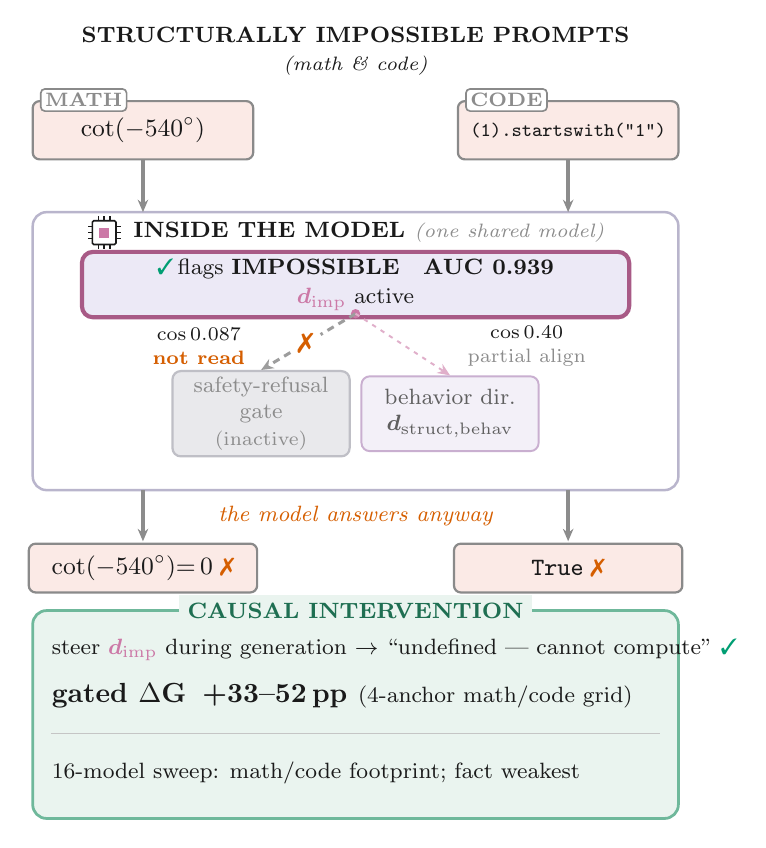
\begin{tikzpicture}[
    >={Stealth[length=4.5pt,width=3.8pt]},
    line width=0.7pt,
    font=\footnotesize,
    every node/.style={inner sep=0pt},
    pcard/.style={rounded corners=2.5pt, line width=0.8pt, draw=cardbd, fill=ppink,
                 align=center, text=ink, inner sep=2pt},
    tab/.style={rounded corners=1.5pt, line width=0.6pt, draw=cardbd, fill=white,
                font=\scriptsize\bfseries, text=gtag, inner sep=1.6pt},
    recog/.style={rounded corners=4pt, line width=1.5pt, draw=herobd, fill=plav,
                 align=center, text=ink, inner sep=2.5pt},
    gate/.style={rounded corners=3pt, line width=0.8pt, draw=gatebd, fill=gatefill,
                 align=center, text=gtag, inner sep=2pt},
    behav/.style={rounded corners=3pt, line width=0.7pt, draw=behavbd, fill=behavfill,
                 align=center, text=ink!70, inner sep=2pt},
    lane/.style={->, line width=1.4pt, gtag},
    domarrow/.style={->, dashed, dash pattern=on 2.6pt off 2.0pt, line width=1.1pt, gtag!85},
    subarrow/.style={->, dashed, dash pattern=on 1.6pt off 2.0pt, line width=0.7pt, dimp!60},
    zhead/.style={font=\footnotesize\bfseries, text=ink},
]
% Frame x:0.15..8.35 (centre 4.25); OUTER prompt/output lanes math x=1.55, code x=6.95.

% ============== TOP HEADER ==============
\node[zhead, align=center] at (4.25,10.02)
     {STRUCTURALLY IMPOSSIBLE PROMPTS\\[0.5pt]{\scriptsize\mdseries\itshape (math \& code)}};

% ============== PROMPT CHIPS (two lanes, with attached MATH/CODE tabs) ==============
\node[pcard, minimum width=2.8cm, minimum height=0.74cm,
      font=\small] (pmath) at (1.55,9.02) {$\cot(-540^\circ)$};
\node[pcard, minimum width=2.8cm, minimum height=0.74cm, font=\scriptsize\ttfamily]
      (pcode) at (6.95,9.02) {(1).startswith("1")};
\node[tab, anchor=west] at ([shift={(3pt,0)}]pmath.north west) {MATH};
\node[tab, anchor=west] at ([shift={(3pt,0)}]pcode.north west) {CODE};

% ============== SHARED MODEL PANEL ==============
\begin{scope}[on background layer]
  \fill[white, rounded corners=5pt] (0.15,4.45) rectangle (8.35,7.98);
\end{scope}
\draw[panelbd, rounded corners=5pt, line width=0.9pt] (0.15,4.45) rectangle (8.35,7.98);
% long, balanced lane arrows: prompts -> panel
\draw[lane] (pmath.south) -- (1.55,7.98);
\draw[lane] (pcode.south) -- (6.95,7.98);
% panel header (chip + title + subtitle)
\node[zhead] (mh) at (4.42,7.72)
     {INSIDE THE MODEL\ \textmd{\scriptsize\itshape\textcolor{gtag}{(one shared model)}}};
\pic at ([xshift=-0.36cm]mh.west) {chip};
% recognition (hero) box -- the shared d_imp signal both lanes produce
\node[recog, minimum width=6.95cm, minimum height=0.74cm] (recog) at (4.25,7.06)
     {{\cmark}\,flags \textbf{IMPOSSIBLE}\quad\textbf{AUC 0.939}\\[1pt]\dimpsym\ active};
% comparator boxes (subordinate to recognition), centred -- NOT under the lanes
\node[gate, minimum width=2.25cm, minimum height=0.95cm] (gate) at (3.05,5.42)
     {safety-refusal\\gate\\[0.5pt]{\scriptsize(inactive)}};
\node[behav, minimum width=2.25cm, minimum height=0.95cm] (behav) at (5.45,5.42)
     {behavior dir.\\\dbehsym};
% ONE shared origin (d_imp signal) -> two DIAGONAL geometry-comparison branches
\fill[dimp] (4.25,6.69) circle (1.7pt);
% dominant route: inactive (light grey), BROKEN with an explicit X in a clean gap
\draw[domarrow,-] (4.25,6.69) -- ($(4.25,6.69)!0.37!(gate.north)$);
\draw[domarrow] ($(4.25,6.69)!0.69!(gate.north)$) -- (gate.north);
\node[font=\normalsize\bfseries] at ($(4.25,6.69)!0.53!(gate.north)$) {\xmark};
\draw[subarrow] (4.25,6.69) -- (behav.north);  % subordinate: down-right
% labels NEXT TO their arrows
\node[font=\scriptsize, align=center, anchor=east] at (2.86,6.28)
     {{\color{ink}\textbf{$\cos 0.087$}}\\[0.5pt]{\color{bad}\bfseries not read}};
\node[font=\scriptsize, align=center, anchor=west] at (5.66,6.28)
     {{\color{ink}$\cos 0.40$}\\[0.5pt]{\color{gtag}partial align}};

% ============== OUTPUT CHIPS (long, balanced arrows; breathing room) ==============
\draw[lane] (1.55,4.45) -- (1.55,3.80);
\draw[lane] (6.95,4.45) -- (6.95,3.80);
\node[font=\footnotesize\itshape, text=bad] at (4.25,4.12) {the model answers anyway};
\node[pcard, minimum width=2.9cm, minimum height=0.62cm, font=\small] (omath) at (1.55,3.46)
     {$\cot(-540^\circ){=}\,0$\;{\xmark}};
\node[pcard, minimum width=2.9cm, minimum height=0.62cm, font=\small] (ocode) at (6.95,3.46)
     {\texttt{True}\;{\xmark}};

% ============== CAUSAL INTERVENTION BAND ==============
\begin{scope}[on background layer]
  \fill[intvfill, rounded corners=5pt] (0.15,0.28) rectangle (8.35,2.92);
\end{scope}
\draw[intvbd, rounded corners=5pt, line width=1.0pt] (0.15,0.28) rectangle (8.35,2.92);
\node[font=\footnotesize\bfseries, text=intvtext, fill=intvfill, inner sep=3pt] at (4.25,2.92)
     {CAUSAL INTERVENTION};
% primary: steer d_imp -> invalidity-aware response (single line)
\node[font=\footnotesize, text=ink, anchor=west] at (0.38,2.42)
     {steer \dimpsym\ during generation $\to$ ``undefined --- cannot compute'' {\cmark}};
% headline result
\node[font=\normalsize\bfseries, text=ink, anchor=west] at (0.38,1.84)
     {gated $\Delta$G\, +33--52\,pp\ \textmd{\footnotesize(4-anchor math/code grid)}};
% divider
\draw[gtag!50, line width=0.4pt] (0.38,1.36) -- (8.12,1.36);
% breadth (16-model sweep), charcoal/readable, single line
\node[font=\footnotesize, text=ink, anchor=west] at (0.38,0.86)
     {16-model sweep: math/code footprint; fact weakest};

\end{tikzpicture}
\end{document}
